\documentclass[10pt,a4paper]{article}
\usepackage[T1]{fontenc}
\usepackage[utf8]{inputenc}
\IfFileExists{lmodern.sty}{\usepackage{lmodern}}{\usepackage{mathptmx}}
\usepackage[margin=2.2cm]{geometry}
\usepackage{graphicx,booktabs,amsmath,amssymb,xcolor,listings,tikz,hyperref,caption}
\usepackage[expansion=false]{microtype}
\usetikzlibrary{positioning,arrows.meta,fit}
\hypersetup{colorlinks=true,linkcolor=blue!50!black,citecolor=blue!50!black,urlcolor=blue!50!black}
\lstdefinestyle{yaml}{basicstyle=\ttfamily\scriptsize,columns=fullflexible,frame=single,framerule=0.3pt,
  keywordstyle=\color{blue!60!black},commentstyle=\color{gray},showstringspaces=false,breaklines=true,
  literate={é}{{\'e}}1 {è}{{\`e}}1 {à}{{\`a}}1}
\newcommand{\CarbonAHystPct}{-0.5}
\newcommand{\CarbonAReactivePct}{8.8}
\newcommand{\CarbonBHystPct}{-2.6}
\newcommand{\CarbonBReactivePct}{3.9}
\newcommand{\CarbonSavingChurn}{91}
\newcommand{\CarbonSavingRetail}{92}
\newcommand{\CostAHystPct}{-0.6}
\newcommand{\CostAReactivePct}{69}
\newcommand{\CostBHystPct}{-1.0}
\newcommand{\CostBReactivePct}{58}
\newcommand{\CostExtraChurn}{5.6}
\newcommand{\CostExtraRetail}{11.1}
\newcommand{\CovData}{5/8}
\newcommand{\CovModel}{5/9}
\newcommand{\CovNonPlan}{21/31}
\newcommand{\CovOps}{9/9}
\newcommand{\CovPlan}{0/7}
\newcommand{\CovSoft}{2/5}
\newcommand{\CovTotal}{21/38}
\newcommand{\FeatEffective}{34}
\newcommand{\FeatLeaves}{50}
\newcommand{\FeatNoEffect}{Airflow, ArgoWorkflows, DataVersioning, ExperimentTracking, Industry40IoT, Kubeflow, Kubernetes, Retail, Serverless, TabularClassification}
\newcommand{\FeatTested}{44}
\newcommand{\JAHyst}{1.000}
\newcommand{\JAOracle}{0.983}
\newcommand{\JAReactive}{1.301}
\newcommand{\JBHyst}{1.009}
\newcommand{\JBOracle}{0.993}
\newcommand{\JBReactive}{1.271}
\newcommand{\JobCarbonAPct}{11}
\newcommand{\JobCarbonBPct}{2}
\newcommand{\MigAHyst}{0.4}
\newcommand{\MigAOracle}{3.1}
\newcommand{\MigAReactive}{102}
\newcommand{\MigBHyst}{0.5}
\newcommand{\MigBOracle}{1.9}
\newcommand{\MigBReactive}{90}
\newcommand{\NConstraints}{10}
\newcommand{\NFeatures}{69}
\newcommand{\NLeaves}{50}
\newcommand{\NLocations}{9}
\newcommand{\NOffers}{27}
\newcommand{\NProfiles}{4}
\newcommand{\NRules}{8}
\newcommand{\RatioMax}{80.6}
\newcommand{\RatioMin}{18.3}
\newcommand{\ScalMaxSeconds}{0.00}
\newcommand{\ScalMaxSteps}{30}

\newcommand{\tool}{\textsf{amlops}}
\renewcommand{\abstractname}{Résumé}\renewcommand{\figurename}{Figure}\renewcommand{\tablename}{Tableau}\renewcommand{\refname}{Références}\renewcommand{\lstlistingname}{Listing}\renewcommand{\today}{25 septembre 2026}

\title{De la connaissance de la variabilité au déploiement multi-cloud souverain~:\\
un DSL low-code pour des pipelines MLOps adaptatifs\\[4pt]
\large Contribution du partenaire industriel au projet ANR AdaptiveMLOps}
\author{Xavier Quesnot\\ GetCaaS, France\\ \texttt{xavier@getcaas.io}}
\date{Version de lecture en français du brouillon v0.1 --- \today\\
\small La version de référence pour soumission est la version anglaise.}

\begin{document}
\maketitle

\begin{abstract}
Les pipelines MLOps doivent être réentraînés en continu pour faire face aux dérives
de données et de concept, et sont de plus en plus exploités sur plusieurs
fournisseurs cloud sous contraintes de coût, de carbone et de souveraineté. Leur
conception mobilise des savoirs répartis entre data scientists, ingénieurs ML et
ingénieurs d'exploitation. En nous appuyant sur la cartographie de la variabilité et
sur l'architecture de référence SkeltyMLOps produites dans le projet ANR
AdaptiveMLOps, nous présentons \tool, un prototype open source qui
(i)~formalise la variabilité MLOps sous forme de modèle de features dont les six
catégories de premier niveau proviennent d'une étude de cartographie antérieure,
complété par des règles de bonnes pratiques documentées~; (ii)~propose un langage
dédié (DSL) YAML à deux niveaux, où un non-expert écrit un profil et des objectifs
tandis qu'un expert affine features, étapes et paramètres~; (iii)~dérive un modèle
de pipeline indépendant de la plateforme selon une approche de ligne de processus
logiciels, y compris des contrats de coordination exécutables~; (iv)~place les
étapes du pipeline entre fournisseurs avec un optimiseur multi-objectif exact et
compile le résultat en Terraform, Argo Workflows et artefacts de CI~; (v)~replace
les services et planifie les réentraînements déclenchés par dérive à l'exécution.
Nous évaluons le prototype sur quatre cas d'étude illustratifs, avec un catalogue
de fournisseurs illustratif et des traces d'environnement synthétiques. Les
artefacts générés réalisent \CovNonPlan{} des activités SkeltyMLOps hors
planification~; \FeatEffective{} des \FeatTested{} features feuilles testables ont un
effet observable sur la sortie, les autres désignant des générateurs manquants. Un
placement statique sensible au carbone réduit le carbone opérationnel de
\CarbonSavingChurn--\CarbonSavingRetail\,\% par rapport à un placement optimisé sur
le seul coût, pour \CostExtraChurn--\CostExtraRetail\,\% de coût en plus. À
l'inverse, le replacement horaire des composants de service apporte peu~: même un
oracle clairvoyant n'améliore l'objectif normalisé que d'environ 2\,\% au plus par
rapport à un placement statique, tandis qu'une politique réactive naïve migre environ
\MigAReactive{} fois par mois et le dégrade de 27 à 30\,\%. Nous discutons de ce que
ces résultats impliquent pour la conception d'outils MLOps adaptatifs et de ce que
des traces industrielles réelles doivent maintenant confirmer.
\end{abstract}

\section{Introduction}
Le MLOps étend le DevOps au développement et à l'exploitation de logiciels intégrant
de l'apprentissage automatique~\cite{kreuzberger2023,sculley2015}. Une fois déployés,
les modèles sont confrontés à des distributions de données changeantes et se
dégradent silencieusement~\cite{gama2014}~; les pipelines embarquent donc du
monitoring, des déclencheurs de réentraînement et du redéploiement. En pratique, ces
pipelines sont assemblés à partir d'outils et de plateformes hétérogènes, et doivent
satisfaire des exigences non fonctionnelles et organisationnelles~: coût, latence,
empreinte environnementale et, en Europe, localisation des données et hébergement
qualifié (par exemple SecNumCloud ou HDS en France).

Le projet ANR AdaptiveMLOps (ANR-24-IAS2-0004) étudie comment l'ingénierie du
domaine (modèles de features, lignes de produits et de processus logiciels) et
l'ingénierie dirigée par les modèles (IDM) peuvent capturer cette variabilité et
assister la conception de nouveaux pipelines. Deux premiers résultats du consortium
cadrent cet article~: une étude de cartographie de la variabilité qui a identifié six
catégories de variabilité et huit exigences de modélisation R1--R8~\cite{elhatimi2025},
et SkeltyMLOps, une architecture de référence fondée sur 38 activités consolidées et
sur des contrats de coordination exécutés par un orchestrateur de
processus~\cite{daoud2025,daoud2026}.

Cet article présente la contribution du partenaire industriel~: une chaîne d'outils
qui transforme cette connaissance en artefacts déployables et redéployables sur une
offre multi-cloud souveraine. Il traite trois questions de recherche~:
\begin{description}
\item[QR1] La connaissance du consortium sur la variabilité et l'architecture de
référence peut-elle piloter un DSL low-code utilisable à deux niveaux d'expertise~?
\item[QR2] Un même modèle DSL peut-il être pivot, c'est-à-dire compilé en
Infrastructure et Platform-as-Code pour plusieurs fournisseurs, avec traçabilité~?
\item[QR3] Qu'apportent les placements multi-fournisseurs statique et dynamique en
coût et en carbone, et au prix de quel risque opérationnel~?
\end{description}

Contributions~: (1) un modèle de features exécutable de la variabilité MLOps, avec
des règles de bonnes pratiques et des correctifs automatiques revalidés~; (2) un DSL
à deux niveaux et un moteur de dérivation fondé sur un processus de base à points de
variation~; (3) une sémantique opérationnelle des contrats de coordination de
SkeltyMLOps~; (4) un optimiseur de placement multi-objectif exact et des générateurs
modèle-vers-texte~; (5) une étude par simulation de politiques de redéploiement, dont
le résultat négatif sur le replacement horaire est, selon nous, instructif. Le code,
les exemples et les scripts d'expériences sont publiés sous licence Apache-2.0~;
chaque chiffre de cet article est produit par le script d'expériences
(section~\ref{sec:dispo}).

\section{Contexte et travaux connexes}
\paragraph{Modèles de features et lignes de processus.} Les modèles de features
(FODA~\cite{kang1990}) décrivent les caractéristiques communes et variables d'une
famille~; leur sémantique se traduit en logique propositionnelle, ce qui permet
l'analyse automatisée~\cite{batory2005,benavides2010}. Les lignes de processus
logiciels appliquent les idées des lignes de produits aux processus, selon l'idée que
les processus logiciels sont eux aussi du logiciel~\cite{osterweil1987}~;
BPMN*~\cite{terenciani2015} annote les modèles de processus avec des points de
variation. L'étude de cartographie du consortium a appliqué cette vision au MLOps et
en a tiré huit exigences~: flot de contrôle et exécution conditionnelle (R1), étapes
optionnelles et alternatives (R2), composition de composants (R3), orchestration
réactive (R4), variabilité multidimensionnelle (R5), extensions spécifiques au
domaine (R6), contraintes et dépendances (R7) et résolution de configuration
(R8)~\cite{elhatimi2025}.

\paragraph{Architectures MLOps et IDM.} Kreuzberger et al.~\cite{kreuzberger2023} et
Najafabadi et al.~\cite{najafabadi2024} synthétisent les composants du MLOps~;
SkeltyMLOps~\cite{daoud2025,daoud2026} organise 38 activités en cinq dimensions
(Plan, Data, Model, Soft, Ops) autour d'un orchestrateur de processus qui exécute des
contrats de coordination composés de tickets, d'événements, de portes (gates) et de
passages de relais (handoffs). DevOpsML~\cite{colantoni2020} tisse modèles de
processus et de plateformes pour le DevOps mais, comme le relève~\cite{elhatimi2025},
sans prise en charge de la variabilité. L'Infrastructure as Code a été largement
étudiée~\cite{rahman2019}, mais l'IaC est généralement écrite fournisseur par
fournisseur plutôt que dérivée d'un modèle de pipeline de plus haut niveau.

\paragraph{Informatique sensible au carbone.} Le décalage temporel des charges
différables vers des heures bas carbone~\cite{wiesner2021} et le modelage
spatio-temporel de la charge dans les centres de données~\cite{radovanovic2023}
montrent que la flexibilité peut réduire les émissions. Nous étudions quelle part de
ce potentiel est atteignable pour des pipelines MLOps sous contraintes de
souveraineté et de latence, et à quel coût de migration.

\section{Vue d'ensemble de l'approche}
La figure~\ref{fig:overview} résume la chaîne d'outils. Une \emph{couche de
connaissance} regroupe le modèle de features, les règles, les profils, le vocabulaire
d'activités SkeltyMLOps et un catalogue de fournisseurs. Un modèle utilisateur (DSL)
est \emph{dérivé} en un pipeline résolu, indépendant de la plateforme~;
l'\emph{optimiseur de placement} associe chaque étape à une offre (fournisseur,
région, type d'instance)~; les \emph{générateurs} produisent l'IaC/PaC~; à
l'exécution, une boucle MAPE-K~\cite{kephart2003} détecte les dérives, ouvre des
tickets sous les contrats et recommande des replacements.

\begin{figure}[t]
\centering
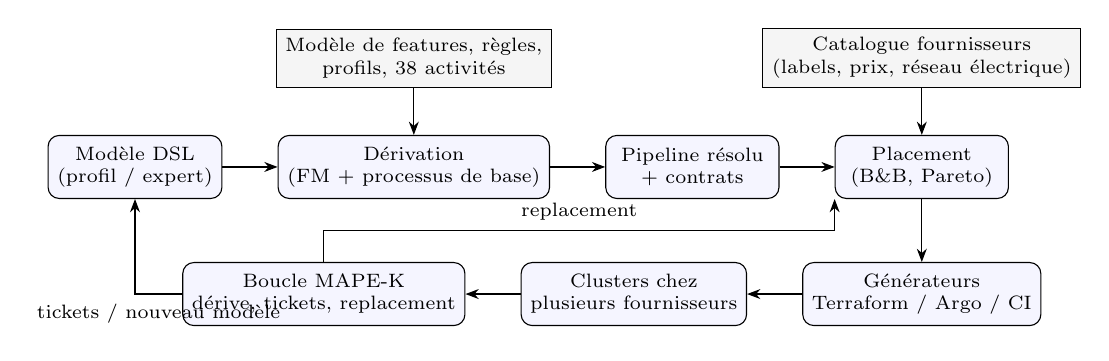
\begin{tikzpicture}[node distance=4mm and 7mm, every node/.style={font=\scriptsize,align=center},
  box/.style={draw,rounded corners,minimum width=22mm,minimum height=8mm,fill=blue!4},
  kb/.style={draw,minimum width=22mm,minimum height=7mm,fill=gray!8}, >=Stealth]
\node[box] (dsl) {Modèle DSL\\(profil / expert)};
\node[box,right=of dsl] (der) {Dérivation\\(FM + processus de base)};
\node[box,right=of der] (pim) {Pipeline résolu\\+ contrats};
\node[box,right=of pim] (pl) {Placement\\(B\&B, Pareto)};
\node[box,below=8mm of pl] (gen) {Générateurs\\Terraform / Argo / CI};
\node[box,left=of gen] (run) {Clusters chez\\plusieurs fournisseurs};
\node[box,left=of run] (mape) {Boucle MAPE-K\\dérive, tickets, replacement};
\node[kb,above=6mm of der] (fm) {Modèle de features, règles,\\profils, 38 activités};
\node[kb,above=6mm of pl] (cat) {Catalogue fournisseurs\\(labels, prix, réseau électrique)};
\draw[->] (dsl)--(der); \draw[->] (der)--(pim); \draw[->] (pim)--(pl); \draw[->] (pl)--(gen);
\draw[->] (gen)--(run); \draw[->] (run)--(mape); \draw[->] (mape.west) -| (dsl.south) node[pos=.25,below]{tickets / nouveau modèle};
\draw[->] (mape.north) -- ++(0,4mm) -| (pl.south west) node[pos=.25,above]{replacement};
\draw[->] (fm)--(der); \draw[->] (cat)--(pl);
\end{tikzpicture}
\caption{La chaîne d'outils \tool.}\label{fig:overview}
\end{figure}

\section{Couche de connaissance}
\paragraph{Modèle de features.} Le modèle de référence compte \NFeatures{} features
(\NLeaves{} feuilles) et \NConstraints{} contraintes transverses. Ses six sous-arbres
de premier niveau sont les catégories de~\cite{elhatimi2025}~: \emph{fonctionnelle}
(tâche ML, prétraitement, optimisation d'hyperparamètres, explicabilité),
\emph{comportementale} (déclencheurs d'entraînement, stratégie de déploiement, porte
humaine), \emph{technique} (orchestrateur, service d'inférence, suivi d'expériences,
versionnement des données, runtime, GPU), \emph{spécifique au domaine}, \emph{non
fonctionnelle} (objectifs, signaux de monitoring) et \emph{organisationnelle}
(localisation, SecNumCloud, cadres de conformité). La contrainte publiée dans le
poster du consortium, \(\neg(\textit{ClassificationBaseline} \wedge
\textit{DimReduction})\), est reprise telle quelle~; les autres encodent des
dépendances sémantiques, par exemple~: un déclencheur sur dérive exige un signal de
dérive~; un système à haut risque au sens de l'AI Act exige une porte humaine et de
l'explicabilité~; l'hébergement HDS implique une contrainte de localisation. Les
features feuilles sont une première proposition du partenaire industriel, à valider
par le consortium.

La complétion de configuration (R8) est une recherche en profondeur sur les features
non décidées, en ordre préfixe, avec évaluation trivaluée de Kleene de toutes les
règles structurelles et contraintes pour l'élagage~; elle renvoie une complétion
minimale (faux d'abord, sauf pour les features marquées par défaut) ou liste les
règles violées.

\paragraph{Règles de bonnes pratiques.} Le savoir-faire qui ne doit pas être une
contrainte dure est stocké sous forme de \NRules{} règles consultatives, chacune avec
une condition, une justification, une source et, si possible, un correctif automatique
exprimé comme un delta de features. Un correctif n'est proposé que si la
configuration résultante est valide. Par exemple, BP01 se déclenche lorsque le
réentraînement est déclenché par dérive sans versionnement des données, ce qui
rendrait les réentraînements automatiques non reproductibles.

\paragraph{Profils.} \NProfiles{} profils sont des configurations partielles nommées
(par exemple \emph{regulated-health-classifier}) qui servent de points d'entrée
low-code.

\section{DSL et dérivation}
La syntaxe concrète est en YAML. Un modèle minimal et un raffinement expert figurent
au listing~\ref{lst:dsl}. La syntaxe abstraite distingue le modèle utilisateur du
pipeline résolu (étapes typées par les activités SkeltyMLOps, déclencheurs, contrats,
objectifs, contraintes de placement).

\begin{lstlisting}[style=yaml,caption={Modèle non expert (haut) et extrait d'un modèle expert (bas).},label=lst:dsl]
pipeline: churn-prediction
profile: tabular-classification-continuous
data: {source: "s3://datalake/crm/churn.parquet", volume_gb: 40}
objectives: {cost: 0.6, carbon: 0.4}
---------------------------------------------------------------
profile: anomaly-detection-edge-iot
best_practices: true            # applique les correctifs automatiques du conseiller
features: {select: [CarbonAware, GPU, HyperparameterTuning, EUResidency]}
placement: {allowed_providers: [scaleway, ovhcloud, outscale], colocate: [[serve, monitor]]}
steps:
  - {id: window_features, kind: transform, activity: D5, after: remove_outliers}
  - {id: train, hours: 3, params: {algorithm: isolation_forest}}
triggers: [{type: drift, detector: ks, threshold: 0.1}]
overrides: {steps.serve.replicas: 3}
\end{lstlisting}

La dérivation (i) complète la configuration à partir du profil et des sélections de
l'utilisateur~; (ii) applique éventuellement les correctifs de bonnes pratiques
valides~; (iii) instancie un processus de base dont les points de variation sont liés
par les features~: \emph{Preprocess} se déploie en une étape par feature de
prétraitement sélectionnée, \emph{Deploy} dépend de la stratégie de déploiement (un
déploiement de test est inséré pour canary, shadow et blue-green), \emph{Serve} est en
ligne ou par lots, \emph{Monitor} porte les signaux sélectionnés~; les étapes
optionnelles (optimisation, explication, approbation humaine) suivent les features
optionnelles~; (iv) fusionne les étapes utilisateur par identifiant, en insérant les
nouvelles dans la chaîne~; (v) applique les surcharges par chemin pointé~; (vi) dérive
les déclencheurs et contrats de coordination à partir des features comportementales,
et les labels de placement à partir des features organisationnelles. Chaque élément
produit enregistre un lien de traçabilité vers sa cause. De nouveaux types d'étapes et
de nouveaux générateurs s'enregistrent via des points d'entrée Python, ce qui couvre
les extensions spécifiques au domaine (R6) sans modifier le DSL.

\paragraph{Contrats de coordination exécutables.} SkeltyMLOps décrit les contrats en
prose~\cite{daoud2026}. Nous leur donnons une sémantique opérationnelle~: un ticket
ouvert sous un contrat n'avance d'une porte à la suivante que lorsque le responsable
de la porte soumet les artefacts requis et, si demandé, une approbation explicite~;
les portes conditionnelles (par exemple \texttt{model.input\_schema !=
api.current\_schema} pour la porte d'impact sur l'API) sont évaluées sur le contexte
du ticket et sautées lorsqu'elles sont fausses~; chaque transition est ajoutée à une
trace auditable. Le contrat de réponse à la dérive dérivé reproduit le scénario
de~\cite{daoud2026}~; les portes humaines ne sont actives que si la feature
\emph{HumanGate} est sélectionnée, ce qu'impose la contrainte liée à l'AI Act.

\section{Placement et génération}
\paragraph{Placement statique.} Chaque étape \(s\) a des besoins en ressources et un
usage mensuel~; chaque offre \(o\) a un prix, une puissance consommée, un PUE, une
intensité carbone du réseau électrique, une latence et des labels. En notant \(x_s\)
l'offre choisie, on minimise
\[
J = w_c\frac{\sum_s \mathrm{coût}(s,x_s)+\sum_{(a,b)}\mathrm{egress}(a,x_a,x_b)}{C_{\mathrm{ref}}}
  + w_g\frac{\sum_s \mathrm{kWh}(s,x_s)\cdot \mathrm{réseau}(x_s)}{G_{\mathrm{ref}}}
  + w_l\frac{\sum_{s\in\mathrm{serve}}\mathrm{lat}(x_s)}{L_{\mathrm{ref}}}
\]
sous contraintes d'adéquation des ressources, de labels requis, de fournisseurs
autorisés, d'épinglages, de groupes de colocalisation et de latence maximale. Les
références sont des sommes de minima par étape, donc \(J\ge 1\) lorsque
\(\sum w=1\), et \(J=1\) signifie que chaque étape est à son optimum individuel. On le
résout exactement par séparation et évaluation (branch and bound) en profondeur dans
l'ordre topologique, avec la borne admissible «~objectif partiel + somme des minima
par étape~» (l'egress est positif ou nul) et une réduction par dominance au niveau
des localisations (pour chaque étape, seule la meilleure offre de chaque localisation
peut être optimale). L'optimalité est vérifiée par force brute dans la suite de tests.
Un balayage des poids donne le front de Pareto coût--carbone.

\paragraph{Génération.} Terraform est produit avec des ressources Scaleway natives
(cluster Kapsule, réseau privé, pools de nœuds, bucket versionné) et des modules à
compléter pour les autres fournisseurs. Pour chaque localisation, un cluster
Kubernetes héberge un WorkflowTemplate Argo contenant les étapes par lots qui y sont
placées~; la porte humaine devient un nœud Argo \texttt{suspend}~; les passages de
relais entre localisations sont des webhooks et capteurs Argo Events~; les
déclencheurs planifiés deviennent des CronWorkflows et les déclencheurs sur dérive des
capteurs alimentés par le monitor~; le service et le monitoring deviennent des
Deployments (ou un InferenceService KServe) avec des ConfigMaps contenant la
politique de dérive et les contrats. Un workflow GitHub Actions régénère les
artefacts, échoue en cas de différence (le modèle est la source de vérité), valide
Terraform et vérifie le schéma des manifestes. Un fichier \texttt{trace.json} relie
chaque fichier aux éléments du modèle et aux activités qu'il réalise.

\paragraph{Adaptation à l'exécution.} Une boucle MAPE-K surveille les lots de
production avec des détecteurs PSI et Kolmogorov--Smirnov à deux échantillons, ouvre
un ticket sous le contrat correspondant et compare le placement courant à un placement
réoptimisé sous les nouvelles conditions. Pour l'étude dynamique, nous considérons le
groupe de service (serve et monitor, colocalisés) et les réentraînements déclenchés par
dérive, ainsi que quatre politiques~: \emph{statique} (placée sur les conditions
moyennes, ne bouge qu'en cas de panne puis revient), \emph{réactive} (suit l'argmin
horaire, réentraîne immédiatement au meilleur endroit), \emph{hystérésis} (ne migre que
si le gain prévu sur une fenêtre d'anticipation dépasse le coût de migration multiplié
par \(1+m\)~; les réentraînements sont décalés dans leur fenêtre de tolérance vers
l'objectif prévu le plus bas) et un \emph{oracle} clairvoyant (programmation dynamique
sur les localisations avec coûts de changement, valeurs futures réelles pour les
réentraînements), qui est une borne inférieure et non une politique réalisable. Les
prévisions sont saisonnières naïves (valeur observée 24\,h plus tôt).

\section{Évaluation}
\paragraph{Protocole.} Quatre cas d'étude illustratifs~: prédiction d'attrition (non
expert, 5 lignes de DSL), aide au triage clinique (profil réglementé, 5 lignes),
maintenance prédictive sur IoT industriel (expert, 28 lignes) et prévision de la
demande en distribution (expert, par lots, 16 lignes). Le catalogue contient
\NOffers{} offres dans \NLocations{} localisations de quatre archétypes de
fournisseurs (deux clouds français, un fournisseur qualifié SecNumCloud/HDS, un
hyperscaler). \emph{Tous les prix, puissances et intensités carbone sont des ordres de
grandeur, pas des tarifs}~; les traces d'environnement (intensité horaire du réseau
avec profils journaliers, creux solaires et bruit AR(1), pannes aléatoires) sont
synthétiques et à graine fixée. Les résultats caractérisent la méthode, pas les
fournisseurs.

\paragraph{QR1 --- Couverture de la connaissance.} Nous basculons chaque feature
feuille dans le contexte d'un profil de référence et vérifions si le modèle dérivé ou
les artefacts générés changent (tableau~\ref{tab:features}). \FeatTested{} des
\FeatLeaves{} feuilles peuvent être basculées de façon cohérente~; \FeatEffective{}
ont un effet observable. Toutes les features comportementales, non fonctionnelles et
organisationnelles ont un effet. Les features inertes sont \FeatNoEffect{}~: elles
révèlent que les générateurs actuels ne ciblent qu'Argo sur Kubernetes, ne produisent
rien pour le versionnement des données ni le suivi d'expériences, et que la tâche ML
et certains domaines ne modifient pas encore le pipeline. Cette mesure fait du modèle
de features un oracle de test de la complétude des générateurs.

\begin{table}[t]\centering\small
\caption{Features feuilles par catégorie~: total, basculables de façon cohérente, et avec effet observable sur la sortie.}\label{tab:features}
\begin{tabular}{lrrr}\toprule
Catégorie & Feuilles & Testées & Avec effet\\\midrule
\csname @@input\endcsname generated/tab_features.tex
\bottomrule\end{tabular}
\end{table}

Côté architecture de référence, les artefacts générés réalisent \CovTotal{} activités
SkeltyMLOps~: Ops \CovOps, Data \CovData, Model \CovModel, Soft \CovSoft, Plan
\CovPlan. Les activités de planification (conception du projet, exigences, conception
de l'architecture) sont humaines par nature et sont soutenues par le DSL lui-même
plutôt que par du code généré~; les activités Data, Model et Soft non couvertes
(collecte et étiquetage des données, expérimentation, développement du code du modèle,
construction et empaquetage) relèvent du travail de développement qu'un DSL de
déploiement laisse volontairement aux utilisateurs.

\paragraph{QR2 --- Modèle pivot.} Le tableau~\ref{tab:abstraction} met en regard la
taille du modèle et les artefacts générés. Un modèle non expert de 5 lignes produit
10 à 11 étapes et environ 400 lignes de configuration Terraform, Argo et CI~; les
modèles experts sont plus longs (ils portent des paramètres) et le ratio descend à
\RatioMin. Ce ratio de lignes n'est qu'un indicateur indirect de l'effort~; il ne
mesure pas la correction du code généré, que nous vérifions en analysant tous les
manifestes, en contrôlant la conformité DNS des noms Argo et la présence de ressources
Terraform natives dans la suite de tests, mais pas encore par un déploiement sur des
clusters réels.

\begin{table}[t]\centering\small
\caption{Taille du modèle et artefacts générés (lignes hors commentaires). Alertes~: règles de bonnes pratiques déclenchées.}\label{tab:abstraction}
\begin{tabular}{lrrrrrr}\toprule
Cas & Lignes DSL & Étapes & Fichiers & Lignes générées & Ratio & Alertes\\\midrule
\csname @@input\endcsname generated/tab_abstraction.tex
\bottomrule\end{tabular}
\end{table}

\paragraph{QR3a --- Placement statique.} Le tableau~\ref{tab:placement} compare
l'optimum aux optima mono-fournisseur et à un placement optimisé sur le seul coût.
Trois observations. (1) L'optimum multi-fournisseurs égale le meilleur optimum
mono-fournisseur (à trois décimales près) dans tous les cas~: la valeur est dans le
choix du bon fournisseur et de la bonne région pour chaque pipeline, pas dans le
découpage d'un pipeline, car l'egress et la colocalisation pénalisent les découpages.
(2) Un mauvais choix coûte cher~: le pire fournisseur unique admissible a un objectif
jusqu'à 35\,\% au-dessus de l'optimum (attrition~: 1,470 contre 1,086). (3) Des poids
sensibles au carbone réduisent le carbone opérationnel de \CarbonSavingChurn\,\%
(attrition) et \CarbonSavingRetail\,\% (distribution) par rapport au placement coût
seul, pour +\CostExtraChurn\,\% et +\CostExtraRetail\,\% de coût~; cet écart tient à
la région moins chère et très carbonée du catalogue et doit être remesuré avec des prix
réels. Pour le cas réglementé, le label HDS ne laisse qu'un seul fournisseur
admissible. Le solveur exact explore 91 à 271 nœuds sur des chaînes de 10 à 30
étapes~; les quasi-égalités entre régions françaises portent ce nombre à
\(3{,}4\times10^5\) nœuds (quelques secondes) pour le cas de maintenance.

\begin{table}[t]\centering\scriptsize
\caption{Placement statique. Coût en EUR/mois, carbone en kgCO\(_2\)e/mois, \(J\) objectif normalisé (1 = optimum par étape).}\label{tab:placement}
\begin{tabular}{lrrrrrrrrr}\toprule
Cas & Fourn. & Coût & Carbone & \(J\) & \(J\) meilleur mono & \(J\) pire mono & Coût (coût seul) & Carbone (coût seul) & Nœuds B\&B\\\midrule
\csname @@input\endcsname generated/tab_placement.tex
\bottomrule\end{tabular}
\end{table}

\begin{figure}[t]\centering
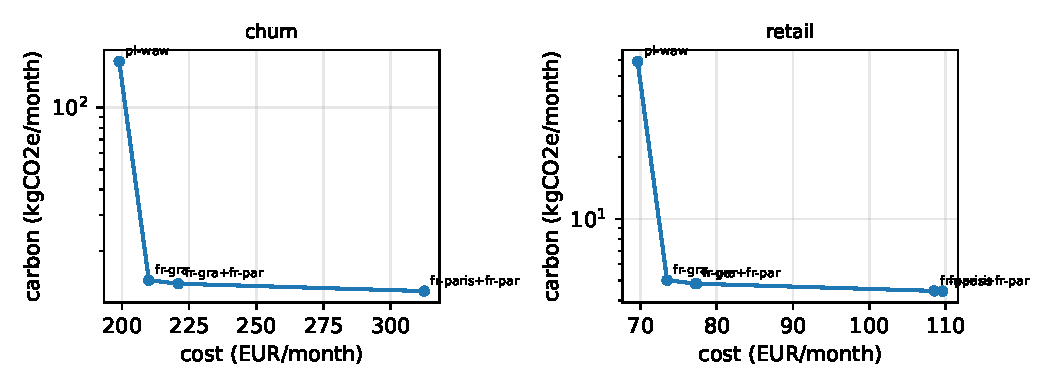
\includegraphics[width=.9\linewidth]{figures/pareto.pdf}
\caption{Fronts de Pareto coût--carbone (balayage des poids)~; les étiquettes indiquent les régions utilisées.}\label{fig:pareto}
\end{figure}

\paragraph{QR3b --- Redéploiement dynamique.} Nous simulons 30 jours (pas horaire)
pour le pipeline de maintenance, avec des poids égaux pour le coût et le carbone,
20 graines, dans deux scénarios~: A, toutes les localisations UE autorisées~; B,
localisations françaises exclues (par exemple une contrainte de localisation vers
d'autres pays de l'UE), ce qui laisse deux localisations de service dont les réseaux
électriques ont des profils journaliers différents. Le tableau~\ref{tab:dynamic}
donne les moyennes sur les graines~; \(J\) est normalisé par la politique statique de
la même graine.

\begin{table}[t]\centering\small
\caption{Politiques dynamiques sur 30 jours (moyenne \(\pm\) écart-type sur 20 graines). Carbone réentr.~: réentraînements déclenchés par dérive uniquement.}\label{tab:dynamic}
\begin{tabular}{llrrrrr}\toprule
Scén. & Politique & Coût (EUR) & Carbone (kg) & Migrations & \(J\) & Carbone réentr. (kg)\\\midrule
\csname @@input\endcsname generated/tab_dynamic.tex
\bottomrule\end{tabular}
\end{table}

Le gain du replacement horaire est faible~: l'oracle clairvoyant n'améliore \(J\) que
de 1,7\,\% (A, \(J=\JAOracle\)) et 0,7\,\% (B, \(J=\JBOracle\)) avec 2 à 3 migrations
par mois. La politique réactive migre \MigAReactive{} (A) et \MigBReactive{} (B) fois
par mois~; elle économise \CarbonAReactivePct\,\% et \CarbonBReactivePct\,\% de
carbone mais augmente le coût de \CostAReactivePct\,\% et \CostBReactivePct\,\%, d'où
\(J=\JAReactive\) et \JBReactive. L'hystérésis évite ces migrations incessantes
(moins d'une migration par mois) mais ne capte pas le gain de l'oracle~:
\(J=\JAHyst\) et \JBHyst. L'ablation (tableau~\ref{tab:ablation}) donne la même image
pour des marges de 0 à 1 et des anticipations de 3 à 12\,h. Une faiblesse identifiée~:
après un déplacement forcé par une panne, l'hystérésis ne revient que si le gain prévu
à court horizon couvre le coût de migration, alors que la politique statique revient
inconditionnellement~; cela explique sa variance carbone plus élevée dans le
scénario~B. Le décalage temporel des réentraînements est le levier le plus
intéressant en relatif~: leur carbone baisse de \JobCarbonAPct\,\% (A) avec une
fenêtre de 12\,h, et l'oracle montre que de meilleures prévisions pourraient
approcher 20\,\%~; les réentraînements ne représentent toutefois qu'une faible part
du total ici.

\begin{table}[t]\centering\small
\caption{Ablation de l'hystérésis, scénario B (10 graines).}\label{tab:ablation}
\begin{tabular}{rrrr}\toprule Marge \(m\) & Anticipation (h) & \(J\) & Migrations\\\midrule
\csname @@input\endcsname generated/tab_ablation.tex
\bottomrule\end{tabular}
\end{table}

\begin{figure}[t]\centering
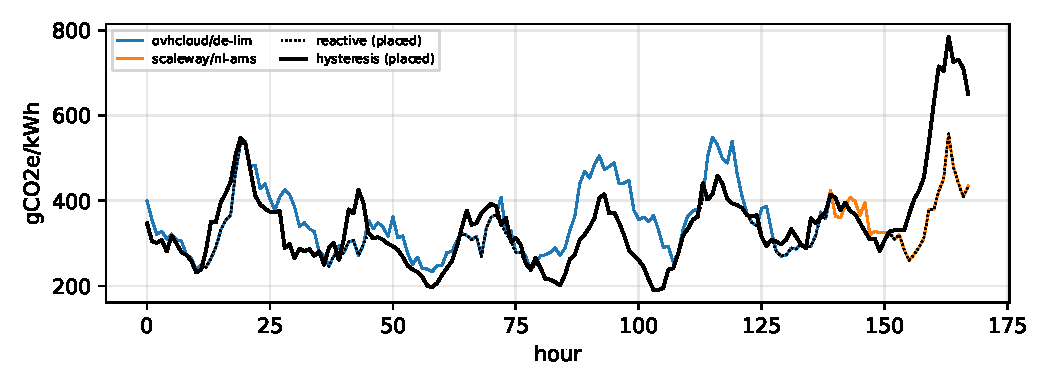
\includegraphics[width=.9\linewidth]{figures/trace_B.pdf}
\caption{Scénario B, première semaine, graine 0~: intensité carbone des deux localisations de service admissibles et intensité subie par le service placé.}\label{fig:trace}
\end{figure}

\section{Discussion}
\paragraph{Pour la conception d'outils.} Sous ces hypothèses, la décision de placement
qui compte est le choix initial du fournisseur et de la région, tenant compte des
contraintes et des objectifs~; il doit être explicite et traçable dès la conception,
ce que fait le DSL. Le replacement dynamique des services de longue durée doit être
conservateur par défaut, déclenché par des événements (pannes, changements de prix ou
de catalogue, réentraînements induits par la dérive) plutôt que par des signaux
horaires~; le décalage temporel des entraînements différables est le levier peu
coûteux. Ces constats portent sur la méthode avec des données synthétiques~; les
ordres de grandeur changeront avec des traces réelles, un état à migrer plus
volumineux ou des régions au réseau plus volatil.

\paragraph{Lien avec les travaux du consortium.} Le prototype réutilise les six
catégories de variabilité, les exigences R1--R8 ainsi que les activités et contrats de
SkeltyMLOps. Il traite R2, R5, R7 et R8 par le modèle de features et la dérivation,
R1 et R4 par les déclencheurs, les portes conditionnelles et les DAG Argo, R3 et R6
par les registres de types d'étapes et de générateurs. Il ne propose pas encore de vue
BPMN ou graphique des processus, ni de métamodèle dans un espace technique IDM standard
(par exemple Ecore)~; ce sont des ponts naturels vers les travaux des partenaires
académiques.

\section{Menaces à la validité}
\emph{Construction}~: \(J\) agrège des critères hétérogènes par des poids et des
références par étape~; le nombre de lignes générées est un indicateur faible de
l'effort~; le carbone est seulement opérationnel et fondé sur la localisation (ni
émissions intrinsèques, ni énergie réseau). \emph{Interne}~: les features feuilles, les
règles et les contraintes sont une proposition de l'auteur, non encore validée par le
consortium~; le coût de migration est une pénalité fixe plus l'egress.
\emph{Externe}~: prix, puissances et intensités carbone sont des valeurs
provisoires et l'environnement est synthétique~; les cas d'étude sont illustratifs et
ne sont pas les cas industriels annoncés dans le projet. \emph{Conclusion}~: 20 graines
donnent des intervalles serrés sur données synthétiques mais ne disent rien de la
variabilité réelle. Les artefacts générés sont analysés et testés unitairement, pas
encore déployés.

\section{Conclusion et feuille de route}
Nous avons présenté \tool, un DSL low-code sensible à la variabilité qui compile des
pipelines MLOps en IaC/PaC multi-fournisseurs et les adapte à l'exécution, en
s'appuyant sur les résultats du consortium AdaptiveMLOps en matière de variabilité et
d'architecture de référence. Prochaines étapes~: (1) revue par le consortium du modèle
de features et des règles~; (2) remplacement du catalogue et des traces par des prix
contractuels et des données réseau mesurées, et déploiement des artefacts générés sur
la plateforme du partenaire industriel~; (3) générateurs pour le suivi d'expériences,
le versionnement des données et d'autres orchestrateurs, guidés par la mesure des
features inertes~; (4) une règle de retour vers la localisation préférée et des
déclencheurs événementiels pour le replacement~; (5) un métamodèle Ecore et une vue
BPMN alignés avec la modélisation en lignes de processus des partenaires
académiques~; (6) une évaluation avec des utilisateurs non experts.

\section*{Disponibilité des données et du code}\label{sec:dispo}
Le code source, les exemples, les tests et le script d'expériences
(\texttt{experiments/run\_all.py}) sont fournis dans le dépôt associé sous licence
Apache-2.0. Tous les tableaux, figures et chiffres de cet article sont produits par ce
script (\texttt{paper/generated/}).

\section*{Remerciements}
Ce travail s'inscrit dans le projet AdaptiveMLOps financé par l'Agence nationale de la
recherche (ANR-24-IAS2-0004).

\section*{Déclaration relative à l'IA générative}
Un assistant fondé sur un grand modèle de langage a été utilisé pour aider à écrire
le code et à rédiger ce texte~; l'auteur a revu la conception, le code, les
expériences et le manuscrit et assume la responsabilité du contenu.

\begin{thebibliography}{99}\small
\bibitem{kreuzberger2023} D.~Kreuzberger, N.~Kühl, S.~Hirschl. Machine Learning Operations (MLOps): Overview, definition, and architecture. \emph{IEEE Access} 11:31866--31879, 2023.
\bibitem{sculley2015} D.~Sculley et al. Hidden technical debt in machine learning systems. \emph{NeurIPS}, 2015.
\bibitem{gama2014} J.~Gama, I.~Žliobaitė, A.~Bifet, M.~Pechenizkiy, A.~Bouchachia. A survey on concept drift adaptation. \emph{ACM Computing Surveys} 46(4), 2014.
\bibitem{elhatimi2025} C.~El Hatimi, V.~Berry, A.-D.~Seriai, V.~Preney, X.~Quesnot, C.~Tibermacine, C.~Urtado, S.~Vauttier. Toward Adaptive MLOps: Variability mapping and modeling. \emph{Journées nationales du GdR GPL}, Pau, 2025. hal-05127859.
\bibitem{daoud2025} C.~Daoud, D.~Azar, J.~Boiché, C.~Urtado, S.~Vauttier. SkeltyMLOps: Orchestrating collaborative MLOps activities. \emph{MLOps25 Workshop, ECAI 2025}, pp.~55--66. hal-05337700.
\bibitem{daoud2026} C.~Daoud, D.~Azar, C.~Urtado, S.~Vauttier. A reference architecture for an orchestrated collaborative MLOps: A ground-up design from literature combining human and LLM expertise. \emph{Future Generation Computer Systems} 185:108700, 2026.
\bibitem{kang1990} K.~C.~Kang, S.~G.~Cohen, J.~A.~Hess, W.~E.~Novak, A.~S.~Peterson. Feature-Oriented Domain Analysis (FODA) feasibility study. CMU/SEI-90-TR-21, 1990.
\bibitem{batory2005} D.~Batory. Feature models, grammars, and propositional formulas. \emph{SPLC}, 2005.
\bibitem{benavides2010} D.~Benavides, S.~Segura, A.~Ruiz-Cortés. Automated analysis of feature models 20 years later: A literature review. \emph{Information Systems} 35(6), 2010.
\bibitem{osterweil1987} L.~Osterweil. Software processes are software too. \emph{ICSE}, 1987.
\bibitem{terenciani2015} M.~Terenciani, D.~M.~B.~Paiva, G.~B.~Landre, M.~I.~Cagnin. BPMN* -- A notation for representation of variability in business process towards supporting business process line modeling. \emph{SEKE}, 2015.
\bibitem{najafabadi2024} F.~Amou Najafabadi, J.~Bogner, I.~Gerostathopoulos, P.~Lago. An analysis of MLOps architectures: A systematic mapping study. \emph{ECSA}, 2024.
\bibitem{colantoni2020} A.~Colantoni, L.~Berardinelli, M.~Wimmer. DevOpsML: Towards modeling DevOps processes and platforms. \emph{MODELS Companion}, 2020.
\bibitem{rahman2019} A.~Rahman, R.~Mahdavi-Hezaveh, L.~Williams. A systematic mapping study of infrastructure as code research. \emph{Information and Software Technology} 108, 2019.
\bibitem{wiesner2021} P.~Wiesner, I.~Behnke, D.~Scheinert, K.~Gontarska, L.~Thamsen. Let's wait awhile: How temporal workload shifting can reduce carbon emissions in the cloud. \emph{Middleware}, 2021.
\bibitem{radovanovic2023} A.~Radovanović et al. Carbon-aware computing for datacenters. \emph{IEEE Transactions on Power Systems} 38(2), 2023.
\bibitem{kephart2003} J.~O.~Kephart, D.~M.~Chess. The vision of autonomic computing. \emph{Computer} 36(1), 2003.
\end{thebibliography}
\end{document}
